\documentclass[tikz, border=1pt]{standalone}

\usepackage{xcolor}
\usetikzlibrary{arrows.meta}
\begin{document}
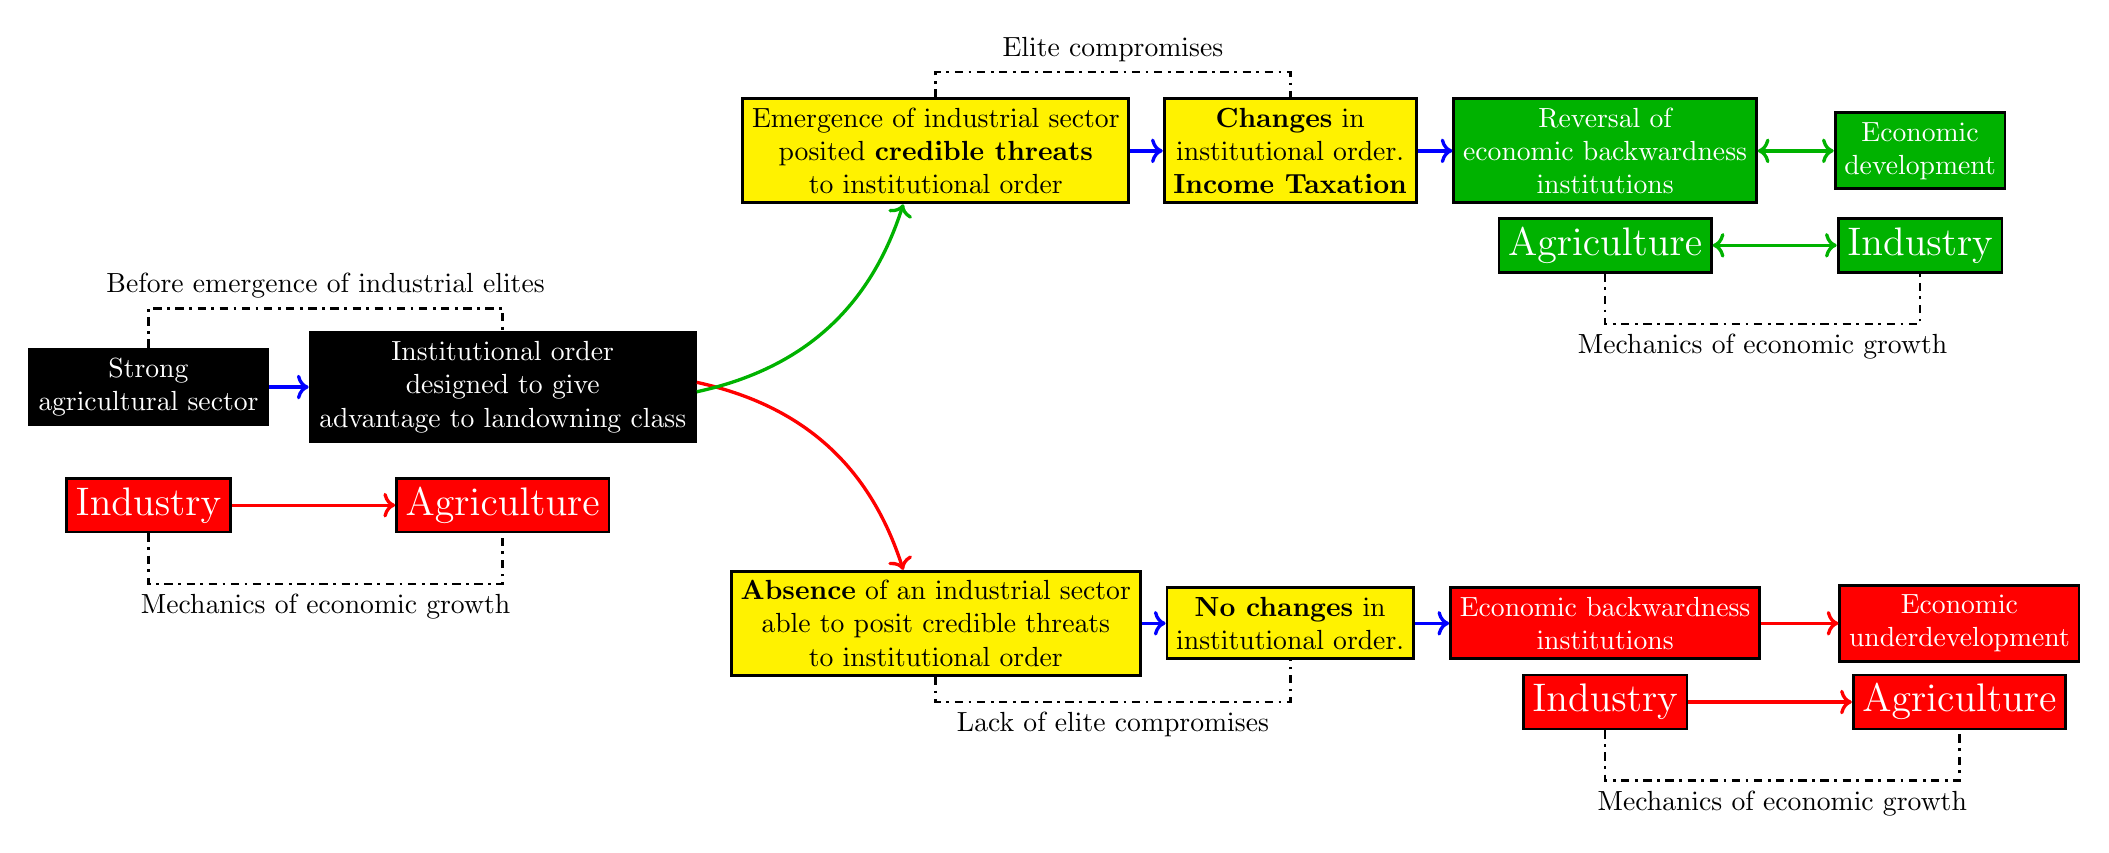
\begin{tikzpicture}[line width=1pt]


% 1










% 2
\node[draw,align=center,fill=black,text=white] (ArgumentA2) at (1,1) {Strong\\agricultural sector};

\node[draw,align=center,fill=red,text=white] (ArgumentA2b) at (1,-0.5) {{\Large Industry}};
\node[draw,align=center,fill=red,text=white] (ArgumentA3b) at (5.5,-0.5) {{\Large Agriculture}};


\node[draw,align=center,fill=black,text=white] (ArgumentB2) at (5.5,1) {Institutional order\\designed to give\\advantage to landowning class};
\node[draw,align=center,fill=yellow,text=black] (ArgumentC) at (11,4) {Emergence of industrial sector\\posited {\bf credible threats}\\to institutional order};
\node[draw,align=center,fill=yellow,text=black] (ArgumentD2) at (15.5,4) {{\bf Changes} in\\institutional order.\\{\bf Income Taxation}};


\draw[dash dot] (ArgumentA2b) -- ++(0,-1) -| (ArgumentA3b)
node[below, near start] {Mechanics of economic growth}; 


%\node[draw,align=center] (ArgumentD23) at (8,4) {Failure to incorporate\\both elites}; 

%\node[draw,fill=red,text=white] (ArgumentE2) at (20.5,4) {Failed state};

\node[draw,fill=black!30!green,text=white,align=center] (ArgumentA4) at (19.5,4) {Reversal of\\economic backwardness\\institutions};
\node[draw,fill=black!30!green,text=white,align=center] (ArgumentB4) at (23.5,4) {Economic\\development};


\node[draw,align=center,fill=black!30!green,text=white] (ArgumentA2c) at (19.5,2.8) {{\Large Agriculture}};
\node[draw,align=center,fill=black!30!green,text=white] (ArgumentA3c) at (23.5,2.8) {{\Large Industry}};


\draw[<->,draw=black!30!green,very thick] (ArgumentB4) to (ArgumentA4);
\draw[->,draw=red,very thick] (ArgumentA2b) to (ArgumentA3b);
\draw[<->,draw=black!30!green,very thick] (ArgumentA2c) to (ArgumentA3c);



\draw[->,draw=blue,very thick] (ArgumentD2) to (ArgumentA4);
%\draw[|-|,draw=blue,thick] (ArgumentC) to (ArgumentD23);

%\draw[->,draw=blue,thick] (ArgumentB4) to (ArgumentE2);




%\draw[->,draw=blue,very thick] (ArgumentB2) to (ArgumentC);
\draw[<-,draw=blue,very thick] (ArgumentD2) to (ArgumentC);
\draw[->,draw=blue,very thick] (ArgumentA2) to (ArgumentB2);

\draw[dash dot] (ArgumentA2) -- ++(0,1) -| (ArgumentB2)
node[above, near start] {Before emergence of industrial elites};


\draw[dash dot] (ArgumentA2c) -- ++(0,-1) -| (ArgumentA3c)
node[below, near start] {Mechanics of economic growth};

\draw[dash dot] (ArgumentC) -- ++(0,1) -| (ArgumentD2) node[above, near start] {Elite compromises}; % here









\node at (6., -1.0) {};






%%%



\node[draw,align=center,fill=yellow,text=black] (ArgumentC_abajo) at (11,-2) {{\bf Absence} of an industrial sector\\able to posit credible threats\\to institutional order};


\node[draw,align=center,fill=yellow,text=black] (ArgumentD2_abajo) at (15.5,-2) {{\bf No changes} in\\institutional order.};


\node[draw,fill=red,text=white,align=center] (ArgumentA4_abajo) at (19.5,-2) {Economic backwardness\\institutions};


\node[draw,fill=red,text=white,align=center] (ArgumentB4_abajo) at (24,-2) {Economic\\underdevelopment};

\node[draw,align=center,fill=red,text=white] (ArgumentA2c_abajo) at (19.5,-3) {{\Large Industry}};
\node[draw,align=center,fill=red,text=white] (ArgumentA3c_abajo) at (24,-3) {{\Large Agriculture}};

\draw[dash dot] (ArgumentC_abajo) -- ++(0,-1) -| (ArgumentD2_abajo) node[below, near start] {Lack of elite compromises}; % here

\draw[dash dot] (ArgumentA2c_abajo) -- ++(0,-1) -| (ArgumentA3c_abajo)
node[below, near start] {Mechanics of economic growth}; 


\draw[<-,draw=red,very thick] (ArgumentB4_abajo) to (ArgumentA4_abajo);
%\draw[->,draw=red,very thick] (ArgumentA2b_abajo) to (ArgumentA3b_abajo);
\draw[->,draw=red,very thick] (ArgumentA2c_abajo) to (ArgumentA3c_abajo);


\draw[->,draw=blue,very thick] (ArgumentD2_abajo) to (ArgumentA4_abajo);


\draw[->,draw=blue,very thick] (ArgumentC_abajo) to (ArgumentD2_abajo);


\path [red,bend left, very thick, ->] (ArgumentB2) edge (ArgumentC_abajo);
\path [black!30!green,bend right, very thick, ->] (ArgumentB2) edge (ArgumentC);


\end{tikzpicture}
\end{document}